\chapter{Architektur und Implementierung}
In den folgenden Abschnitten wird zunächst die allgemeine Architektur der Implementierung erklärt. Anschließend werden die wichtigsten Klassen vorgestellt, sodass der Trainings- und Evaluationsprozess nachvollzogen werden können.
\section{Architektur}

\begin{figure}[h]
    \centering
    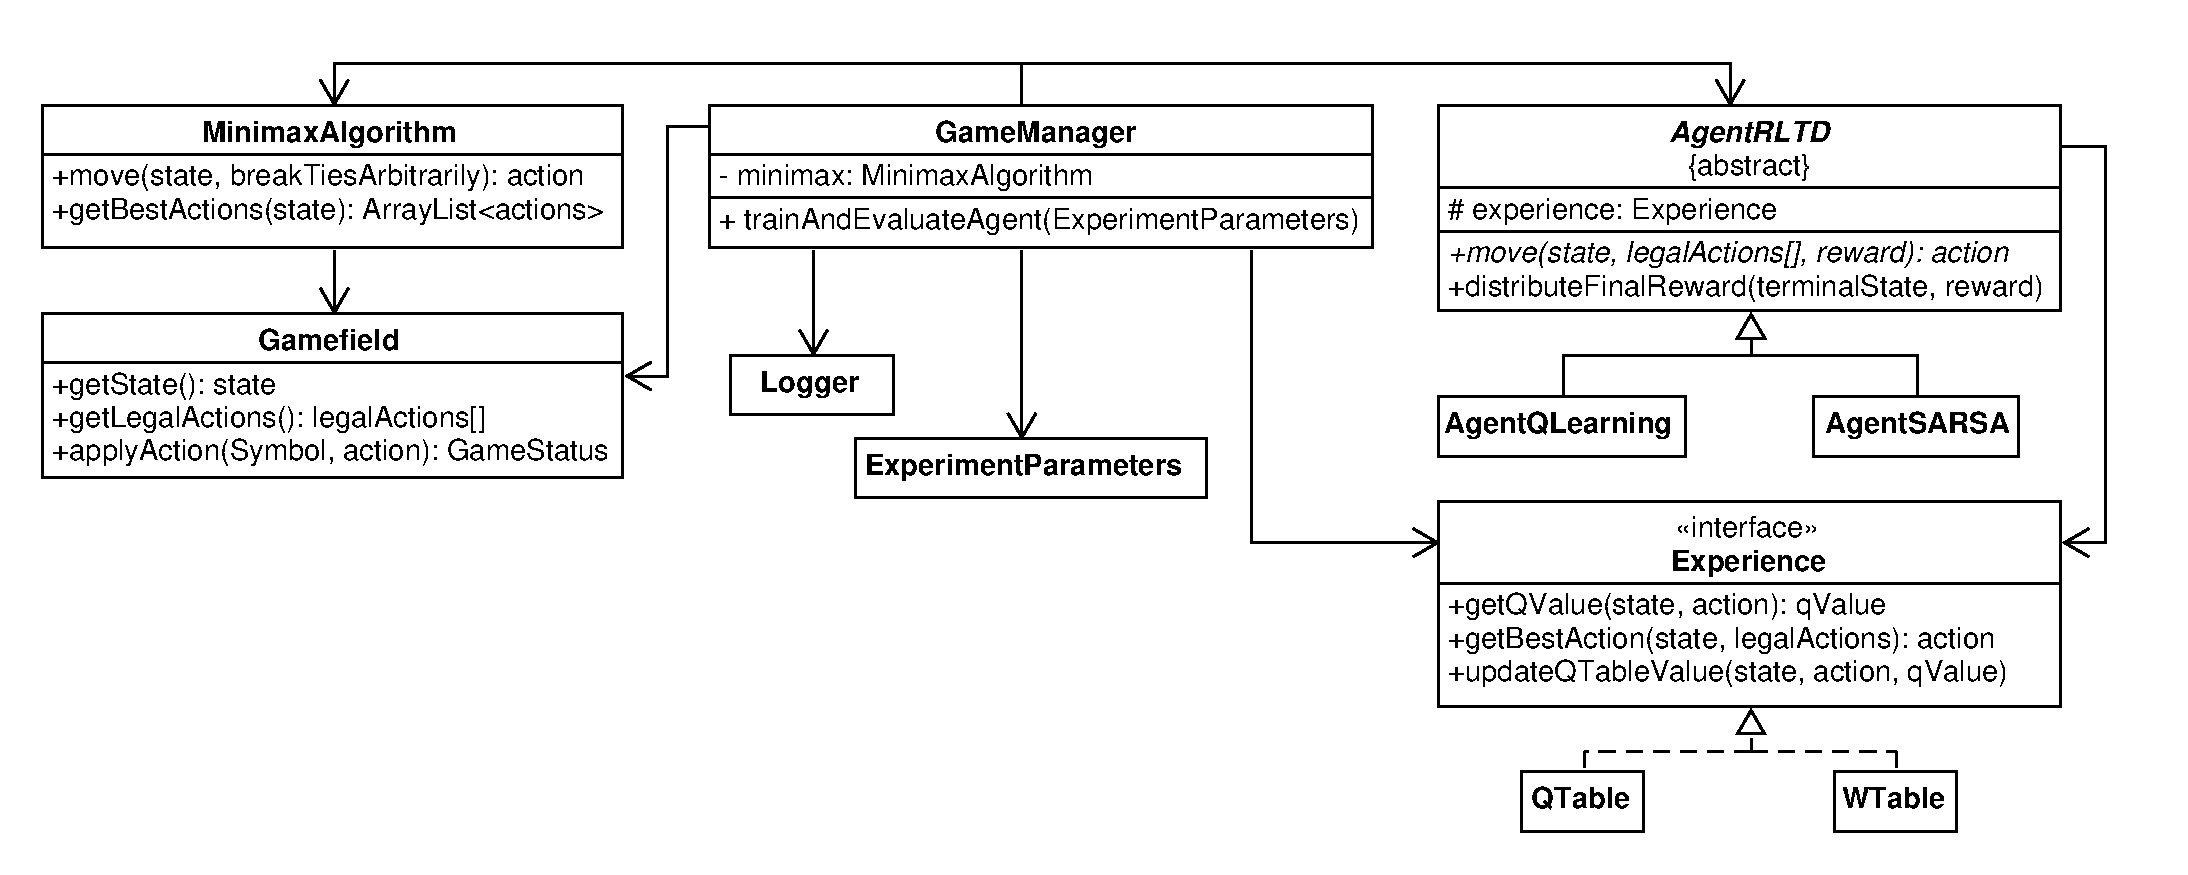
\includegraphics[width=\linewidth]{uml/uml_architektur.pdf}
    \caption{Grobe Übersicht der wichtigsten Klassen und deren Interaktion}
    \label{fig:uml_architektur}
\end{figure}

In \cref{fig:uml_architektur} ist eine Übersicht der wichtigsten Klassen.
Das UML-Diagramm stellt keinen Anspruch an Vollständigkeit, sondern dient der Vermittlung eines grundlegenden Verständnisses für die wichtigsten Bestandteile der Anwendung sowie deren Interaktion. 
Der GameManager ist die zentrale Klasse, die alle anderen Klassen verbindet, um Training und Evaluation der Agenten durchzuführen.  
Auf Basis, der in ExperimentParameters definierten Werte erstellt der GameManager zwei Agenten und weist diesen eine gemeinsame Experience Instanz zu. 
Die beiden Agenten werden mittels \splay trainiert und anschließend in Evaluationsspielen getestet. 
Zur Bewertung der Agenten verwendet der GameManager den Minimax-Algorithmus. 
Währenddessen erstellt der GameManager Log-Dateien auf deren Basis die Auswertung erfolgt.
Einerseits CSV-Dateien, die zum Plotten der Konvergenz und Berechnen der Spielstärke verwendet werden.
Zum anderen Dateien, wie im \cref{chap:meta}, die für Training und Evaluation verwendete Experimentparameter und Spielergebnisse enthalten. 
In den folgenden Abschnitten werden die Bestandteile genauer betrachtet.

Für die Implementierung wurde Java 16 und somit die derzeit aktuellste Java Version verwendet. 
Um die volle Kontrolle über die Implementierung der Agenten zu haben, wurden keine zusätzlichen Bibliotheken eingebunden. 
Die einzige Ausnahme ist die Bibliothek Apache CommonsCSV, die zur Erstellung von CSV-Dateien genutzt wird. 
Der Source-Code und die Dokumentation der Anwendung sowie Verwendungshinweise werden bereitgestellt auf \href{http://github.com/JonasBingel/ThesisHSMZ-RLTicTacToe-Java}{Github.com/JonasBingel}
\section{Gamefield}
Die Klasse Gamefield implementiert das Tic-Tac-Toe Spielfeld, wie es in \cref{chap:ttt_encoding} beschrieben wurde. 
Gamefield verwaltet pro Symbol ein Bitboard. 
Die Bitboards $B_X$ und $B_O$ wurden umgesetzt mittels der Java BitSet-Klasse, die einen Vektor von Bits verwaltet. 
Zudem implementiert die BitSet-Klasse die klassischen Logikoperationen, sodass die beschriebene Methodik zur Erfassung der legalen Aktionen und Gewinnprüfung umgesetzt werden können. 

In der Anwendung werden möglichen Aktionen und die Binärrepräsentation $B_{s}$ eines Zustands jeweils in einem int zur Basis 10 gespeichert.
Der primitve Datentyp int umfasst 32 Bits und ist somit ausreichend, um die 18 Bit von $B_{s}$ zu verwalten.  \cref{listing:getState} zeigt die Berechnung von $B_{s}$ und somit die Implementierung der \cref{eq:bitboard_bs}. 
Bevor die zu den Bitboards zugehörigen Zahlen addiert werden, erhält $B_X$ mittels LSHIFT den beschriebenen Offset von 9 Bit, d.h. der Spielfeldgröße, damit keine Überschneidung von $B_X$ und $B_O$ auftritt.

\begin{listing}[h]
\caption{getState-Methode zur Berechnung von $B_S$}
\label{listing:getState}
\inputminted{java}{04_Artefakte/03_Listings/getState.java}
\end{listing}
\section{Minimax}
\begin{figure}
    \centering
    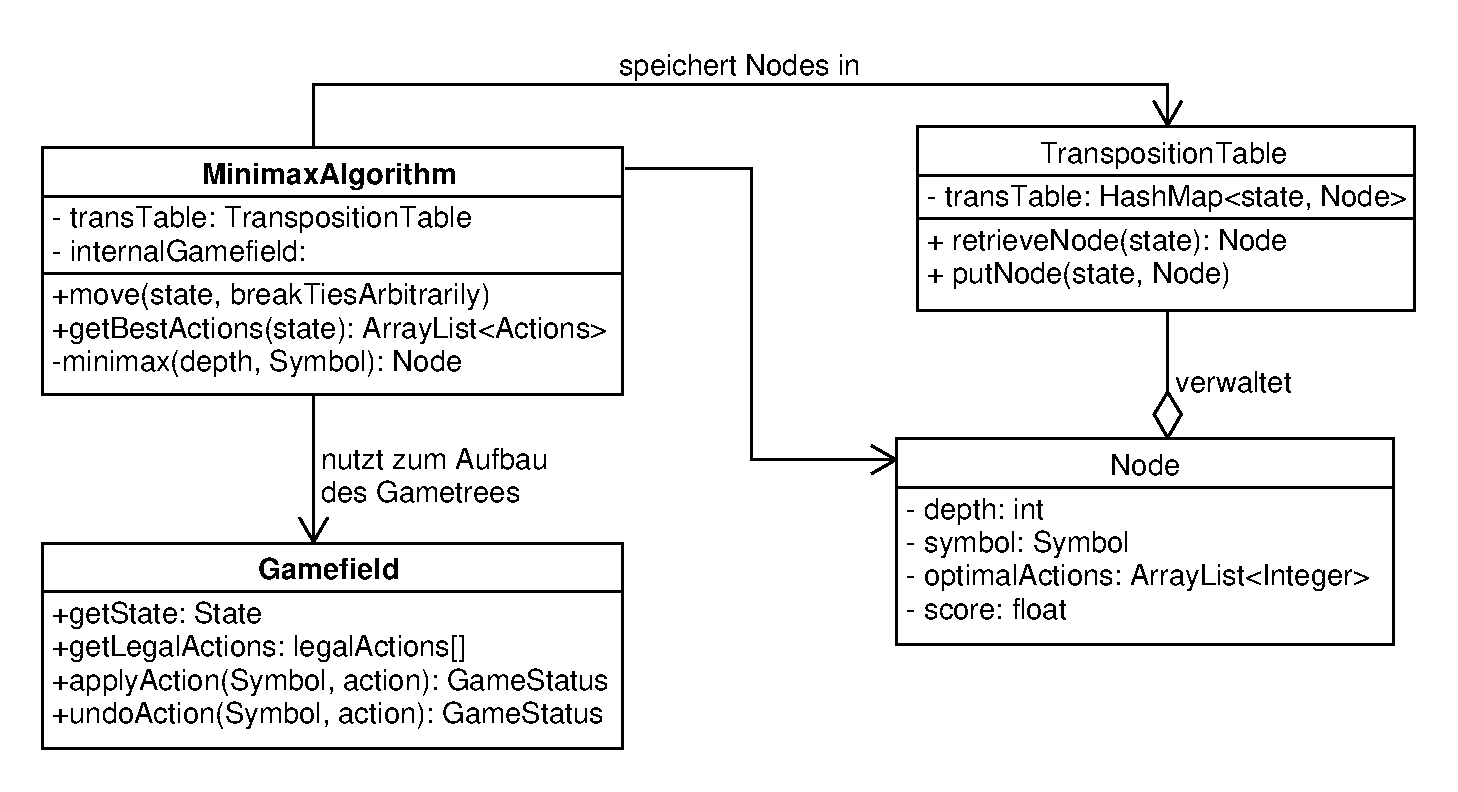
\includegraphics[width=\textwidth]{04_Artefakte/01_Abbildungen/uml/uml_minimax.pdf}
    \caption{MinimaxAlgorithm und verbundene Klassen}
    \label{fig:uml_minimax}
\end{figure}

\cref{fig:uml_minimax} zeigt die wichtigsten Bestandteile der MinimaxAlgorithm-Klasse sowie deren Interaktion mit anderen Klassen.
MinimaxAlgorithm implementiert den Minimax-Algorithmus aus \cref{sec:minimax} und dient der Evaluation der Agenten. 
Einerseits wird während des Trainings geprüft, ob die vom Agenten gewählten Aktionen optimal sind. 
Andererseits ist Minimax ein Gegner im Rahmen der Evaluationsspiele, um die Spielstärke der Agenten zu messen. 

Die Klasse bietet dafür zwei Methoden. 
Für die Bewertung der Aktionen des Agenten gibt es die getBestActions-Methode. 
Diese gibt alle gleich optimalen Aktionen zu einem Zustand zurück, sodass geprüft werden kann, ob die vom Agenten gewählte Aktion ein Element dieser Liste und somit optimal ist. 
Die move-Methode gibt für einen Zustand eine der optimalen Aktionen zurück, sodass Minimax als Gegner genutzt werden kann. 
Dabei kann als zweiter Parameter übergeben werden, ob bei mehreren gleich optimalen Aktionen die Aktion mit dem niedrigsten Index oder eine zufällige ausgewählt werden soll. 
Da in den Evaluationsspielen möglichst viele unterschiedliche Zustände betrachtet werden sollen, wird die Option für nichtdeterministisches Spiel genutzt.

Der Spielbaum wird konstruiert durch die minimax-Methode, die in Listing \cref{chap:minimax_listing} dargestellt ist. 
Mit jedem Aufruf wird ein weiterer Knoten (engl. Node) dem Spielbaum hinzufügt. 
In der minimax-Methode wird der aktuelle Zustand sowie die legalen Aktionen des intern verwalteten Spielfelds abgerufen. 
Eine der legalen Aktionen wird auf das Spielfeld angewendet und für den resultierenden Zustand wird erneut Minimax aufgerufen. 
Wird ein Terminalknoten erreicht, wird die letzte Aktion rückgängig gemacht und die nächste legale Aktion ausgeführt. 
Dies erfolgt rekursiv, bis alle Äste des Spielbaums konstruiert wurden. 
Jeder Knoten des Spielbaums entspricht einem Zustand des Spielfelds und wird repräsentiert durch eine Node-Instanz. 
Die Nodes werden unter der eindeutigen Nummer $B_{s}$ des zugehörigen Zustands in einer Transposition table gespeichert. 

Im Rahmen der Minimax-Methode werden zudem die Attribute der Node des aktuellen Zustands auf Basis der darauf folgenden Nodes aktualisiert. 
Dies beinhaltet die Anpassung der zu erwartenden Utility und die darauf basierende Auswahl der optimalen Aktionen, wobei Symbol X der maximierende und O der minimierende Spieler ist. 
Als Bewertungsfunktion verwendet Minimax ebenfalls die in \cref{sec:TDL_TTT} vorgestellte Rewardfunktion mit Depth Penalty.
\section{Reinforcement Learning Komponenten}
In den folgenden Abschnitten werden die Komponenten beschrieben, die \acl{RL} implementieren. 
Dies umfasst die Agenten für \bothAlgs sowie deren Lerndaten in Form der Q- und \wtable.

\subsection{\qlearning und \sarsa Agenten}
Da \bothAlgs eng verwandte \ac{TDL} Algorithmen sind, wurde eine abstrakte Klasse RLTDAgent erstellt, von der die konkreten Agenten abgeleitet werden. 
Neben dem Vorteil der Redundanzvermeidung nutzen AgentQLearning und AgentSARSA ein einheitliches Interface und können in den Trainings- und Evaluationsmethoden untereinander ausgetauscht werden.

Der Unterschied der beiden Algorithmen liegt in deren Vorgehen in jedem Zeitschritt, weshalb die move-Methode als abstrakt deklariert wurde. 
\cref{listing:moveQL} und \cref{listing:movesarsa} zeigen die Implementierung der move-Methode des AgentQLearning und AgentSARSA. 
Wie in \cref{chap:vergleich} erklärt, unterscheiden sie sich in zwei Aspekten. 
Einerseits in der Aktion, die jeweils für das Update verwendet wird. 
Bei \qlearning ist dies immer Aktion mit dem höchsten  \qValue und bei \sarsa die Aktion, die der Agent wirklich durchführt. 
Andererseits liegt der Unterschied darin, dass \qlearning das \ac{TD} Update durchführt, bevor es die Aktion für den Zustand $S'$ wählt. 
Da im Fall von \acs{TTT} kein Zustandswechsel möglich ist, bei dem ein Zustand $S$ sein eigener Folgezustand $S'$ ist, könnte das \acl{TD} Update auch nach der Aktionswahl durchgeführt werden. 
Dadurch reduziert sich der Unterschied auf die Wahl der Aktion für das Update. 
Auf diese Reduktion wurde verzichtet, um die Algorithmen wie vorgestellt zu implementieren und den Unterschied deutlich im Source-Code darzustellen. Beide move-Methoden implementieren die $\epsilon$-greedy-Policy \cite[S. 27f.]{suttonReinforcementLearningIntroduction2018}.

\begin{listing}[p]
\caption{move-Methode des Agent Q-Learning}
\label{listing:moveQL}
\inputminted{java}{04_Artefakte/03_Listings/move_qlearning.java}
\end{listing}

\begin{listing}[p]
\caption{move-Methode des Agent Sarsa}
\label{listing:movesarsa}
\inputminted{java}{04_Artefakte/03_Listings/move_sarsa.java}
\end{listing}

\subsection{Lerndaten}
\begin{figure}
    \centering
    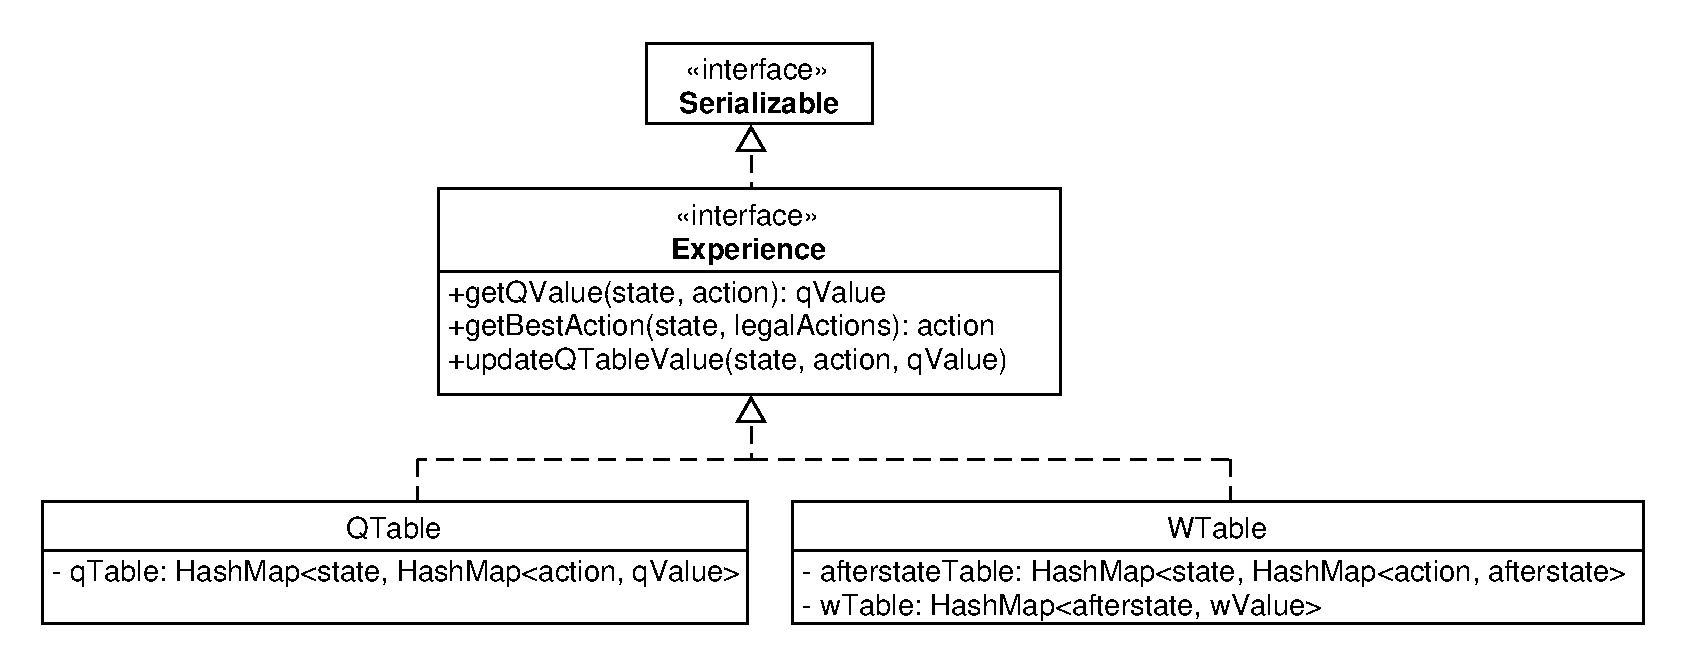
\includegraphics[width=\textwidth]{04_Artefakte/01_Abbildungen/uml/uml_experience.pdf}
    \caption{Experience Interface und implementierende Klassen}
    \label{fig:uml_experience}
\end{figure}

Die gesammelte Erfahrung des Agenten wird in der Anwendung durch das Experience Interface implementiert, das in \cref{fig:uml_experience} dargestellt ist. 
Da der Agent die Lerndaten in Form einer \qtable oder \wtable organisieren kann, bietet das Experience Interface dem Agenten einheitliche Methoden zum Zugriff auf die Lerndaten. 
Die in \cref{sec:afterstates} beschriebene Abbildung der \ac{SA Tupel} auf den resultierenden Afterstate, wird so ebenfalls vom Agenten entkoppelt und erfolgt in der Klasse WTable.

Eine Experience Instanz wird nicht durch einen Agenten selbst erzeugt, sondern im Konstruktor übergeben. 
Diese Implementierung hat zwei Gründe. 
Zum einen ist es notwendig, damit zwei Agenten im Rahmen von \splay gemeinsam eine Experience Instanz füllen können. 
Zum anderen verdeutlicht die Trennung, dass die Erfahrung kein inhärenter Bestandteil eines Agenten ist, sondern diese nur vom Agenten verwendet werden. 
Der Unterschied eines trainierten und untrainierten Agenten eines Algorithmus besteht, abgesehen von den Hyperparametern, in der Erfahrung, auf die jeweils zugegriffen wird. 
Aus diesem Grund implementiert Experience das Java Interface Serializable, wodurch Erfahrungen als Datei exportiert und importiert werden können, sodass Agenten erneut geladen werden können, um weitere Tests durchzuführen. 
In der Implementierung sind \qtable und der \afterstateTable beide mittels geschachtelten HashMaps umgesetzt, für die als Schlüssel jeweils die eindeutigen Zustände $B_{S}$ und Aktionen verwendet werden.

Im vorgestellten Pseudocode von \bothAlgs werden die \qValues aller \ac{SA Tupel} vor der ersten Episode willkürlich initialisiert. 
Dies setzt voraus, dass eine Liste aller legalen \ac{SA Tupel} vorliegt. 
Stattdessen werden in der Implementierung die \qtable und \wtable dynamisch konstruiert. 
Bei jedem Aufruf der move-Methode eines Agenten reicht dieser den aktuellen Zustand sowie die legalen Aktionen zur Initialisierung weiter. 
Dies ermöglicht die Erfassung der Zustandsanzahl, die der Agent im Rahmen des Trainings besucht hat. 
Im Konstruktor kann der initiale \qValue übergeben werden. 
In dieser Arbeit wird ausschließlich 0 verwendet. 
\section{GameManager}
Die Klasse GameManager ist zuständig für Training und Evaluation der Agenten sowie das Logging.
In \cref{fig:uml_sequence} ist der vereinfachte Ablauf des Trainings mit klassischem \splay für AgentSARSA dargestellt.
Für jedes Training wird ein neues Gamefield erzeugt und Experimentparameter definiert, auf deren Basis Experience und Agenten initialisiert werden. 
Zu Beginn jeder Episode werden die Hyperparameter der Agenten entsprechend der Experimentparameter aktualisiert. 
Anschließend wird ein Spiel gestartet und in jedem Zug werden der Zustand und die legalen Aktionen des Gamefields abgerufen. 
Beginnend mit X werden abwechselnd die move-Methoden der Agenten aufgerufen, in dessen Rahmen der direkte Reward, $r=0$, ausgegeben wird. 
Die zurückgegebene Aktion wird auf das Gamefield angewandt. 
Nach Ende des Spiels, wird der Reward mit Depth Penalty für die letzte Aktion beider Agenten verteilt und das Spielfeld zurückgesetzt. 
Das Training mit alternierendem \splay folgt dem gleichen Ablauf.
Innerhalb eines Batchs werden die Hyperparameter des nicht lernenden Agenten so gesetzt, das dieser mit der Greedy-Strategie spielt und bei Aufruf seiner move-Methode kein \ac{TD} Update durchführt.
Im Anschluss an das Training werden beide Agenten im Rahmen von Evaluationsspielen bewertet und die Experience Instanz wird als Datei serialisiert.

\begin{figure}[h]
    \centering
    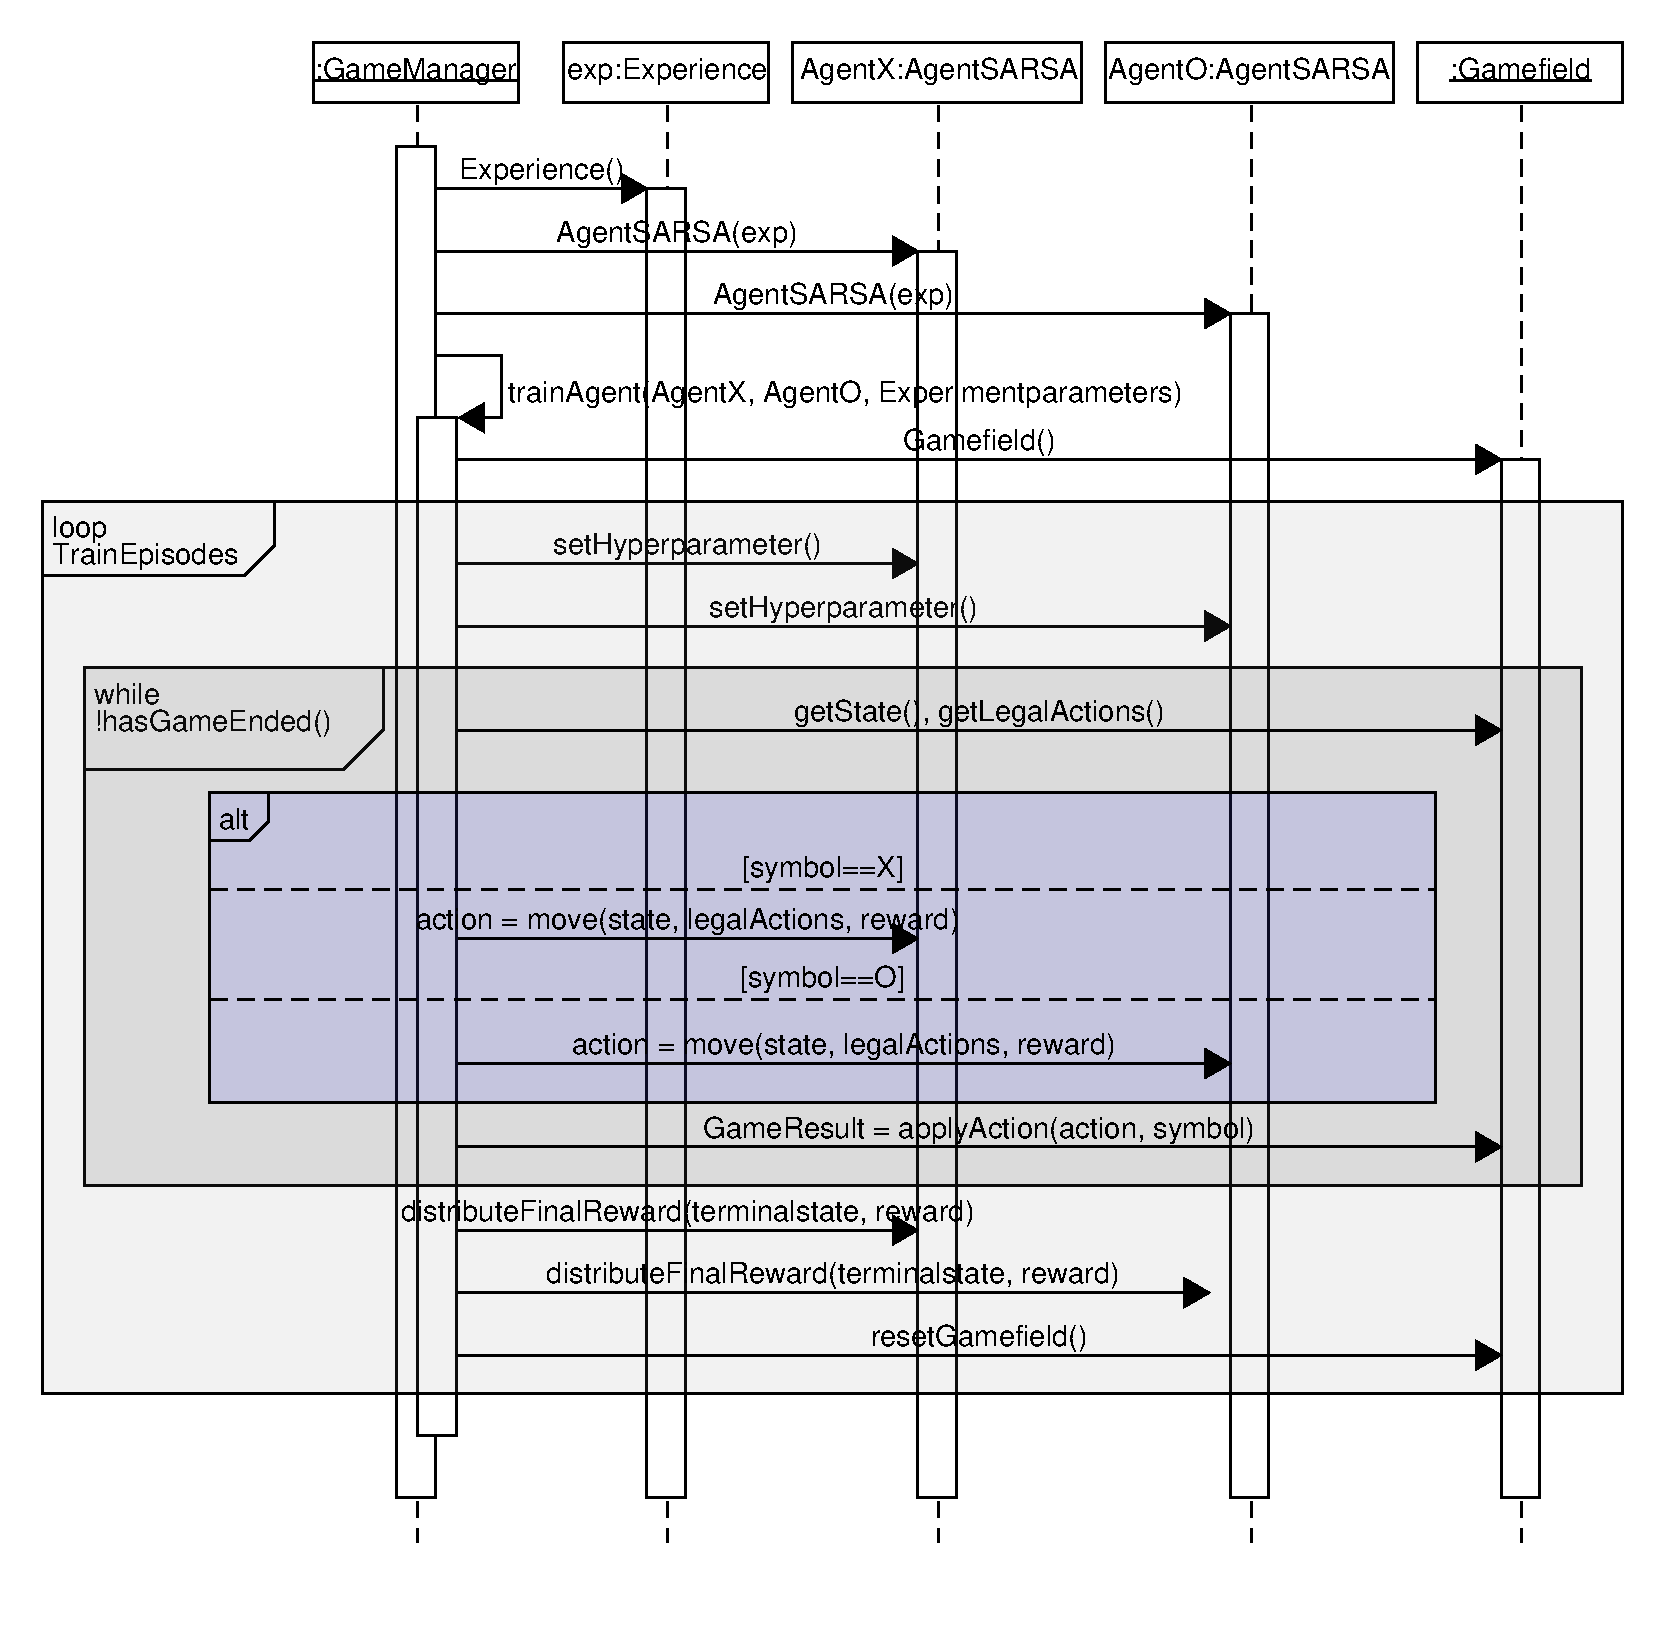
\includegraphics[width=\linewidth]{04_Artefakte/01_Abbildungen/uml/uml_sequence.pdf}
    \caption{Vereinfachte Darstellung des Trainingsablaufs mit klassischem \splay}
    \label{fig:uml_sequence}
\end{figure}